%\section{Closing Remarks}
\section{Conclusions and Limits}

\begin{frame}{\thesection. \insertsection}
	We present a system capable of automatically landing a MAV on a moving GV, tested experimentally at speeds up to $50$ km/h %moving at 50 km/h.
	\begin{itemize}
		\item Built using low cost off-the-shelf components
		\vspace{0.5cm}
		\item Using a visual fiducial marker and a mobile phone on the GV + long-range WiFi link
		\vspace{0.5cm}
		%\item Using a linear Kalman filter for relative position estimation.
		\item Classical design blocks: PN and PD guidance laws, Kalman filter for relative state estimation
		%\item Code openly available at : ...
	\end{itemize}
\end{frame}

% ----------------------------------------------------------------------

%\begin{frame}{\thesection. \insertsection}
%\begin{frame}{Limits}
%	%What can we do better?
%	\begin{itemize}
%		\item Going Faster and being more robust at high speed
%			\begin{itemize}
%				\item effect of air flow at ? %Integrate the car's airflow model into the control law.
%				\item Strategies to stick to landing pad
%			\end{itemize}
%			\item Trust in control logic with complex sensor pipelines\dots
%		%\item Remove the need for a mobile phone.
%		%\item Add a system to get the MAV to stick to the landing pad e.g. magnets or motors supporting negative thrust.
%		%\item Go faster!
%	\end{itemize}
%\end{frame}



\begin{frame}{Limits and Future Directions}
	%Automatic landing of a micro aerial vehicle (MAV) on a moving ground vehicle (GV)
	%\begin{itemize}
	%	\item Package delivery, logistics
	%	\item Long distance deployments (battery savings)
	%	\item Benefits from heterogeneous capabilities (ex: monitoring) %Automatic fleet management
	%\end{itemize}
	\begin{figure}[ht]
        \begin{minipage}[t]{0.46\linewidth}
            \centering
            \includemedia[
			%width=0.4\linewidth,
	  		%totalheight=0.225\linewidth,
	  		%activate=pageopen,
			%final,
			playbutton=plain, %none,
	  		passcontext,  %show VPlayer's right-click menu
	  		addresource=figures/50kmh.mp4,
	  		flashvars={
	    		%important: same path as in `addresource'
	    		source=figures/50kmh.mp4
			}
	]{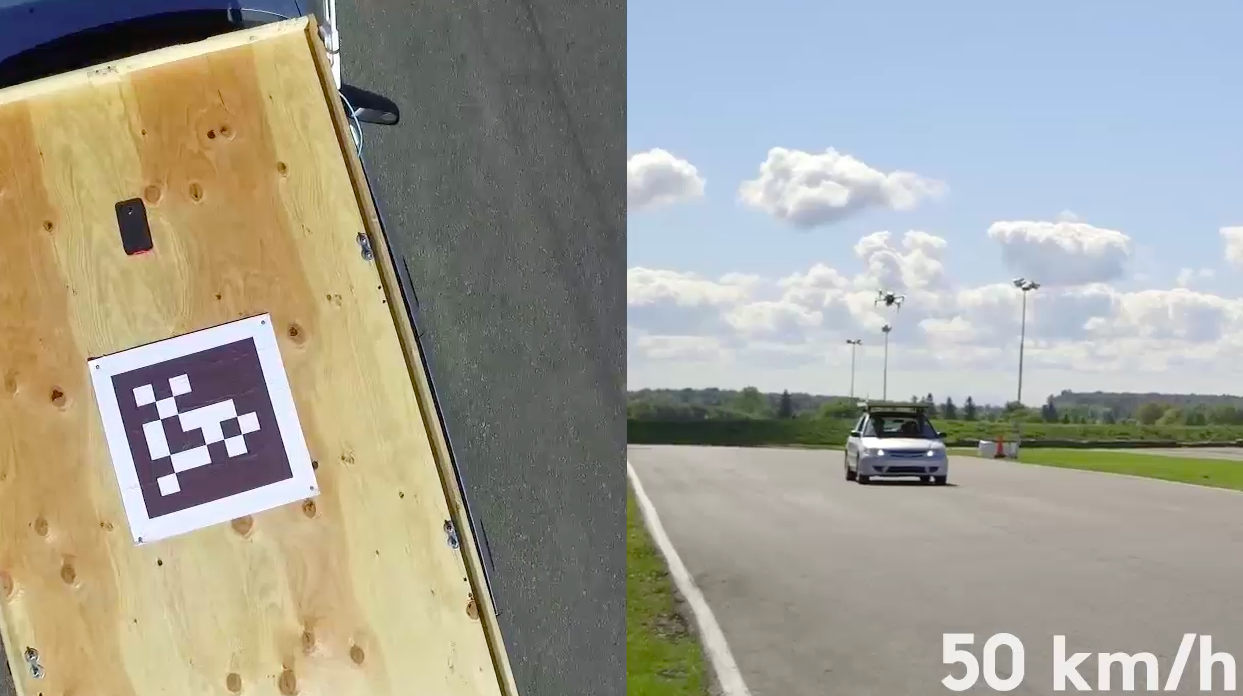
\includegraphics[width=\textwidth]{figures/50kmhPoster.png}}{VPlayer.swf}
            %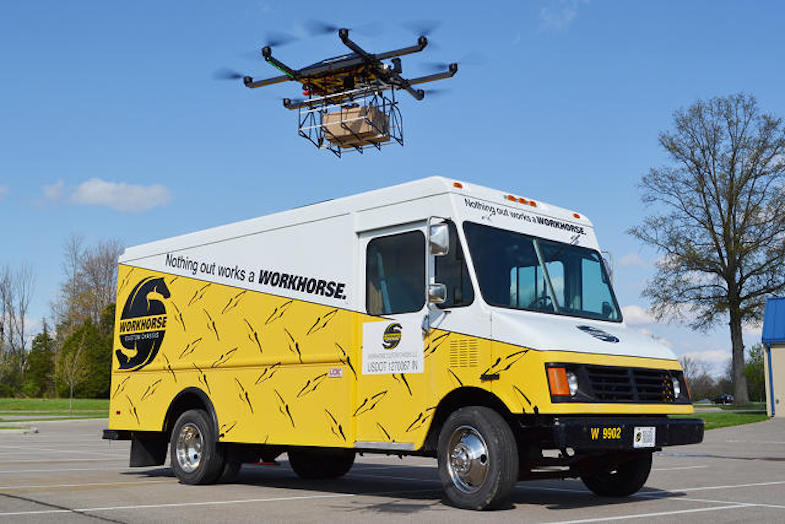
\includegraphics[width=\textwidth]{figures/ups.jpg}\\
            %\caption{MAV assisted deliveries by truck}
            Air flow effects, more rigorous model-based approach at high speed
            %\begin{itemize}
            %\item 
            %\item Stick to landing pad
            %\end{itemize}
            %\label{fig:a}
        \end{minipage}
        \hspace{0.5cm}
        \begin{minipage}[t]{0.46\linewidth}
            \centering
            \includemedia[
			%width=0.4\linewidth,
	  		%totalheight=0.225\linewidth,
	  		%activate=pageopen,
			%final,
			playbutton=plain, %none,
	  		passcontext,  %show VPlayer's right-click menu
	  		addresource=figures/crash.mp4,
	  		flashvars={
	    		%important: same path as in `addresource'
	    		source=figures/crash.mp4
			}
	]{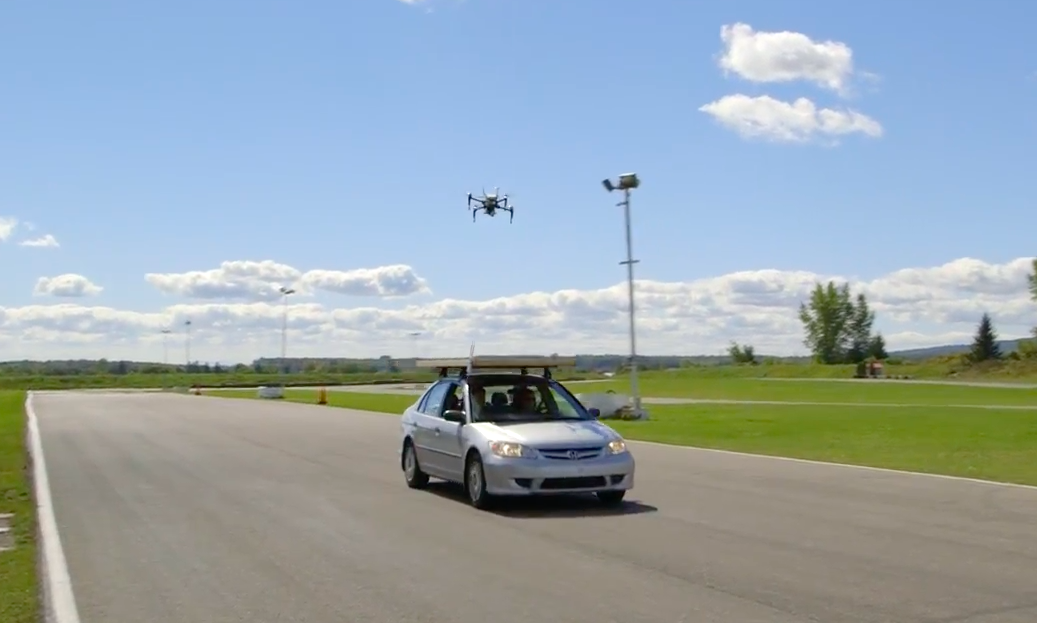
\includegraphics[width=\textwidth]{figures/crashPoster.png}}{VPlayer.swf}
            %\caption{Truck based long range MAV deployments}
            %Truck based long range MAV deployments
            Trust in ad-hoc logic interfacing complex perception pipelines, external components
            %\label{fig:b}
        \end{minipage}
     	\end{figure}
\end{frame}


%\begin{frame}{\thesection. \insertsection}	
%	Why did it slip at $50$ km/h ?
%	\begin{enumerate}
%		\item Close to top speed of the MAV 
%		\item We introduced a small delay before motor cutoff to allow the MAV to straighten out.
%		\item At these speeds, airflow around the car becomes significant.
%	\end{enumerate}
%	The last two points combined give the MAV just enough lift to slide backwards.
%\end{frame}